\documentclass[12pt]{article}
\usepackage{fullpage,islsymb,graphicx}

\DefineVerbatimEnvironment{code2}{Verbatim}{tabsize=0,xleftmargin=0.5in,numbers=left,firstnumber=last,commandchars=\!\{\}}

\def\Rank{\operatorname*{\textbf{Rank}}}
\newcommand{\symm}{{\mbox{\bf S}}}  % symmetric matrices
\newcommand{\herm}{{\mbox{\bf H}}}  % Hermitian matrices
\newcommand{\lorentz}{{\mbox{\bf Q}}}  % lorentz cone
\newcommand{\ones}{\mathbf 1}

\title{\cvx Users' Guide\\\large version 0.85 (alpha)}
\author{Michael Grant\\\texttt{mcgrant@stanford.edu} 
\and Stephen Boyd\\\texttt{boyd@stanford.edu}
\and Yinyu Ye\\\texttt{yyye@stanford.edu}}
\bibliographystyle{alpha}

\begin{document}
\maketitle
\tableofcontents

\section{Introduction}

\subsection{What is \cvx?}

\cvx is a modeling system that supports \emph{disciplined convex 
programming}. Disciplined convex programs (DCPs) are convex optimization
problems that adhere to a limited set of construction rules that enable
them to be analyzed and solved efficiently. The set of DCPs
includes most well-known classes of convex programs, including
linear programs (LPs), (convex) quadratic programs (QPs), second-order
cone programs (SOCPs), and semidefinite programs (SDPs).
In fact, almost any convex optimization problem
that one is likely to encounter in practice, even 
nondifferentiable problems, can be represented relatively
easily as a DCP. For background on convex optimization, see the book 
\emph{Convex Optimization} \cite{BV:04}; for more discussion 
of disciplined convex programming, see \cite{GBY,Gra:04}.

\cvx is implemented in Matlab \cite{MATLAB}, effectively
turning Matlab into an optimization modeling language.
Model specifications are constructed using common Matlab
operations and functions, and standard Matlab code can be
freely mixed with those specifications. This combination
makes it simple to perform the calculations
needed to form optimization problems, or to process the
results obtained from their solution. For example, it is easy
to compute an optimal trade-off curve
by forming and solving a family of optimization problems
by varying the constraints. As another example, \cvx can
be used as a component of a larger system that uses convex
optimization, such as a branch and bound method,
or an engineering design framework.

\cvx converts problems into a canonical form that is compatible
with interior-point algorithms. Problems involving nondifferentiable 
functions can be automatically transformed into equivalent smooth forms,
enabling them to be solved without the loss in performance typically
associated with nondifferentiability.
A significant amount of problem sparsity and block
structure is revealed to the underlying solver, which can be
exploited to improve performance.

\cvx comes with a base library of convex
and concave functions and convex sets that can be used
directly in the construction of DCPs. New functions can
be added in three ways:
\begin{itemize}
\item Existing functions 
can be combined according to the disciplined convex programming 
composition rules.
\item A function can be described as the optimal value 
of an partially specified convex optimization problem, expressed
in the \cvx modeling language.
\item A smooth convex or concave function can be described by
specifying its convexity and monotonicity properties and supplying
code to compute its value, gradient, and Hessian.
\end{itemize}
This last option is not available in this alpha version (see \S\ref{sec:version} below).
The base library also includes several useful convex sets, such as the
positive semidefinite matrix cone. In the future, \cvx will also allow
new sets to be added in two ways:
\begin{itemize}
\item The set can be described using the \cvx modeling language in the
form of a convex feasibility problem.
\item Code to compute the value, gradient, and Hessian
of a barrier function for the set may be provided.
\end{itemize}

\cvx was designed and implemented by Michael Grant, with input
from Stephen Boyd and Yinyu Ye \cite{GBY}. It
incorporates ideas from earlier work by 
L\"{o}fberg \cite{YALMIP}, 
Dahl and Vandenberghe \cite{CVXOPT}, 
Crusius \cite{Cru:02}, 
Wu and Boyd \cite{SDPSOL},
and many others.
The modeling language follows
the spirit of AMPL \cite{AMPL} or GAMS \cite{GAMS}; unlike
these packages, however, \cvx is designed to fully exploit convexity.
The specific method for implementing \cvx in Matlab
draws heavily from YALMIP \cite{YALMIP}.
We hope to implement a version of \cvx in Python,
as part of the CVXOPT system \cite{CVXOPT}, in the near future.

\subsection{What is disciplined convex programming?}

\cvx is designed to support \emph{disciplined convex programming},
a methodology for constructing convex optimization problems
proposed by Michael Grant, Stephen Boyd, and Yinyu Ye \cite{GBY}.
This name was chosen to indicate that the treatment of convex
programming as a distinct discipline, one in which convexity is an
advance requirement. In other words, \cvx is designed to support the formulation and
construction of optimization problems that the user 
intends \emph{from the outset} to be convex.
To that end, \cvx imposes a limited
set of conventions or rules, which we call the \emph{DCP ruleset},
that enable it to verify convexity
and convert problems to solvable form reliably and efficiently.
Problems that violate the ruleset are rejected, even when
convexity of the problem is obvious to the user.
That is not to say that such problems cannot be solved; they
just need to be rewritten in a conforming manner.

A detailed description of the DCP ruleset is given in \S\ref{sec:rules},
and it is important for anyone who wishes to actively use
\cvx to understand it. The ruleset is simple 
to learn, drawn from basic principles of convex analysis,
and resembles the practices of those who study and use
convex optimization. In addition, the ruleset actually \emph{enables}
considerable benefits, such as the automatic conversion of
problems to solvable
form and full support for nondifferentiable
functions. In practice, we have found that
disciplined convex programs still closely resemble
their natural mathematical forms.

\subsection{About this version}
\label{sec:version}

In this first version of \cvx,
SeDuMi \cite{Stu:99} is the only core solver supported.
SeDuMi is an interior-point solver written in Matlab for 
LPs, SOCPs, and SDPs.
Future versions of \cvx will support other solvers, such as
MOSEK \cite{MOSEK}, and a general purpose solver we are developing.

Because SeDuMi only solves LPs, SOCPs, and SDPs, this
version of \cvx can only handle functions that can be represented
using these problem types, and problems that can be reduced to 
these problem forms. Thus the current version includes such
functions as $\ell_1$, $\ell_2$,
and $\ell_\infty$ norms, maximum, minimum, absolute value,
quadratic forms, square root,
and maximum and minimum eigenvalue of a symmetric matrix,
as well as a few obscure functions such as the 
sum of the largest $k$ entries of a vector.
Some useful functions that are \emph{not} supported in
the current version include
exponential and log, powers other than 2 and $0.5$,
entropy, log-sum-exp, and the log-determinant of a matrix.

Several other features planned for
\cvx are \emph{not} supported in this 
release, including user-defined smooth functions, user-defined sets,
and geometric programming.
We hope to extend \cvx to handle these fairly soon.

Any feedback and criticism you might
have about this software, particularly at this early stage,
would be greatly appreciated.
Please contact Michael Grant (\texttt{mcgrant@stanford.edu}) or
Stephen Boyd (\texttt{boyd@stanford.edu}) with your comments. If
you discover a bug, please notify us at the above addresses; and
if at all possible, please include:
\begin{itemize}
\item the code and data that caused the error;
\item a copy of any error messages that it produced;
\item the version number of Matlab that you are running; and
\item the name and version of the operating system you are using.
\end{itemize}

\section{A quick start}
\label{sec:quickstart}

Once you have installed \cvx (see \S\ref{s-installing}), you can
start using \cvx by entering a \cvx \emph{specification} into a
Matlab script or function, or directly from the command prompt.
To delineate \cvx specifications from surrounding Matlab code,
they are preceded with the statement
\verb@cvx_begin@ and followed with the statement
\verb@cvx_end@. A specification can
include any ordinary Matlab statements, as well as
special \cvx-specific commands for declaring primal and dual 
optimization variables and specifying constraints and
objective functions.

Within a \cvx specification, optimization variables have no numerical
value, but are special Matlab objects.   
This enables Matlab to distinguish
between ordinary commands and \cvx objective
functions and constraints. As Matlab reads a \cvx specification,
it builds an internal representation of the
optimization problem. If it encounters a
violation of the rules of disciplined convex programming
(such as an invalid use of a composition rule or an invalid
constraint), an error message is generated.
When Matlab reaches 
the \verb@cvx_end@ command, it completes the conversion of
the \cvx specification to a canonical form,
and calls the underlying solver 
(which is SeDuMi, in this first version).

If the optimization is successful,
the optimization variables declared in the \cvx specification
are converted from objects to ordinary Matlab numerical values
that can be used in any further Matlab calculations. In addition,
\cvx also assigns a few other related Matlab variables.
One, for example, gives the status of the problem (\ie, whether an
optimal solution was found, or the problem was determined to be 
infeasible or unbounded).  Another gives the optimal value
of the problem. Dual variables can also be assigned.

This processing flow will become more clear as we introduce
a number of simple examples. We invite the reader to actually follow
along with these examples in Matlab, by running the \verb@quickstart@
script found in the \verb@examples@ subdirectory of the \cvx distribution. 
For example,
if you are on Windows, and you have installed the \cvx distribution
in the directory \verb@D:\Matlab\cvx@, then you would type
\begin{code}
	cd D:\Matlab\cvx\examples
	quickstart
\end{code}
at the Matlab command prompt.
The script will automatically print key excerpts of its code, and
pause periodically so you can examine its output. (Pressing ``Enter''
or ``Return'' resumes progress.) 
The line numbers accompanying the code excerpts in this
document correspond to the line numbers in the file \verb@quickstart.m@.

\subsection{Least-squares}
\label{sec:leastsquares}

We first consider the most basic convex optimization problem,
least-squares.
In a least-squares problem, we seek $x \in \R^n$
that minimizes $\|Ax-b\|_2$, where $A\in \R^{m \times n}$ is
skinny and full rank (\ie, $m\geq n$ and $\Rank (A)=n$).
Let us create some test problem data for $m$, $n$, $A$, and $b$ in Matlab:
\begin{code2}[firstnumber=15]
	m = 16; n = 8;
	A = randn(m,n);
	b = randn(m,1);
\end{code2}
(We chose small values of $m$ and $n$ to keep the output readable.)
Then the least-squares solution  $x=(A^TA)^{-1}A^Tb$ is easily
computed using the backslash operator: 
\begin{code2}[firstnumber=20]
	x_ls = A \ b;
\end{code2}
Using \cvx, the same problem can be solved as follows:
\begin{code2}[firstnumber=23]
	cvx_begin			!label{code:beg}
	    variable x(n);		!label{code:var}
	    minimize( norm(A*x-b) );	!label{code:obj}
	cvx_end				!label{code:end}
\end{code2}
(The indentation is used for purely stylistic reasons and is optional.) 
Let us examine this specification line by line:
\begin{itemize}
\item Line~\ref{code:beg} creates a placeholder for the
new \cvx specification, and prepares Matlab to accept 
variable declarations, constraints, objective function, and so forth. 
\item Line~\ref{code:var} declares \verb@x@
to be an optimization variable of dimension $n$. \cvx
requires that all problem variables be declared before they are used in
objective functions or constraints. 
\item Line~\ref{code:obj}
specifies an objective function to be minimized; in this case,
the Euclidean or $\ell_2$-norm
of $Ax-b$. 
\item Line~\ref{code:end} signals the end of the \cvx specification,
and causes it to be solved.
\end{itemize}
The backslash form is clearly simpler---there is no reason to use \cvx
to solve a simple least-squares problem. But this
example serves as sort of a ``Hello world!'' program in \cvx;
\ie, the simplest code segment that actually does something useful.

If you were to type \verb@x@ at the
Matlab prompt after line~\ref{code:var} but
before the \verb@cvx_end@ command, you would see something
like this:
\begin{code}
	x =
	    cvx affine expression (8x1 vector)
\end{code}
That is because within a specification, variables have no
numeric value; rather, they are Matlab objects 
designed to represent problem variables and expressions
involving them. Similarly, 
because the objective function \verb@norm(A*x-b)@ 
involves a \cvx variable, it does not have a numeric value either; 
it is also represented by a Matlab object.

When Matlab reaches the \verb@cvx_end@ command, the least-squares
problem is solved,
and the Matlab variable \verb@x@ is overwritten
with the solution of the least-squares problem, \ie, $(A^TA)^{-1}A^Tb$.
Now \verb@x@ is an ordinary length-$n$ numerical vector, identical
to what would be obtained in the traditional approach, at least to
within the accuracy of the solver. In addition, two additional Matlab
variables are created:
\begin{itemize}
\item \verb@cvx_optval@, which contains the value of the objective
function; \ie, $\|Ax-b\|_2$;
\item \verb@cvx_status@, which contains a string describing the
status of the calculation. In this case, \verb@cvx_status@
would contain the string \verb@Solved@. See Appendix \ref{sec:status}
for a list of the possible values of \verb@cvx_status@ and their meaning.
\end{itemize}
All three of these quantities, \verb@x@, \verb@cvx_optval@, and
\verb@cvx_status@, may now be freely used in other Matlab
statements, just like any other numeric or string values.\footnote{If you type
\texttt{who} or \texttt{whos} at the command prompt, you may see other, unfamiliar
variables as well. Any variable that begins with the prefix \texttt{cvx\_} is 
reserved for internal use by \cvx itself, and should not be changed.}

There is not much room for error in specifying a simple least-squares
problem, but if you make one, you will get an error or warning message.
For example, if you replace line~\ref{code:obj} with
\begin{code}
	maximize( norm(A*x-b) );
\end{code}
which asks for the norm to be maximized, you will get an error message
stating that a convex function cannot be maximized (at least in
disciplined convex programming):
\begin{code}
??? Error using ==> maximize
Disciplined convex programming error:
Objective function in a maximization must be concave.
\end{code}

\subsection{Bound-constrained least-squares}
\label{sec:bcls}

Suppose we wish to add some simple upper and
lower bounds to the least-squares problem above: \ie, we wish to solve 
\begin{equation}
\begin{array}{ll}
\mbox{minimize} & \|Ax-b\|_2\\
\mbox{subject to} & l \preceq x \preceq u,
\end{array}
\label{eq:bcls}
\end{equation}
where $l$ and $u$ are given data, vectors with the same dimension
as the variable $x$.
The vector inequality $u \preceq v$ means componentwise, \ie,
$u_i \leq v_i$ for all $i$. We can no longer use the simple
backslash notation to solve this problem, but it can be transformed into
into a quadratic program (QP), which can be solved without difficulty
if you have some form
of QP software available. 

Let us provide some numeric values for \verb@l@ and \verb@u@:
\begin{code2}[firstnumber=47]
	bnds = randn(n,2);
	l = min( bnds, [] ,2 );
	u = max( bnds, [], 2 );
\end{code2}
Then if you have the Matlab
Optimization Toolbox \cite{MATOPT}, you can use the \verb@quadprog@ function
to solve the problem as follows:
\begin{code2}[firstnumber=53]
	x_qp = quadprog( 2*A'*A, -2*A'*b, [], [], [], [], l, u );
\end{code2}
This actually minimizes the square of the norm, which is the same as
minimizing the norm itself. In contrast, the \cvx specification is given by
\begin{code2}[firstnumber=59]
	cvx_begin
	    variable x(n);
	    minimize( norm(A*x-b) );
	    subject to			!label{code:subjto}
	        x >= l;			!label{code:lower}
	        x <= u;			!label{code:upper}
	cvx_end
\end{code2}
Three new lines of \cvx code have been added to the \cvx specification:
\begin{itemize}
\item The \verb@subject to@ statement on line~\ref{code:subjto} does nothing---\cvx
provides this statement simply to make specifications more readable. 
It is entirely optional.
\item Lines~\ref{code:lower} and~\ref{code:upper}
represent the $2n$ inequality constraints $l \preceq x \preceq u$.
\end{itemize}
As before, when the \verb@cvx_end@ command is reached, the problem
is solved, and the numerical solution is assigned to the variable
\verb@x@. Incidentally, \cvx will 
\emph{not} transform this problem into a QP by squaring the objective;
instead, it will transform it
into an SOCP. The result is the same, and the transformation
is done automatically.

In this example, as in our first, the \cvx specification is 
longer than the Matlab alternative. On the other hand, it is easier
to read the \cvx version and relate it to the original problem.
In contrast, the \verb@quadprog@ version requires us to know in advance
the transformation to QP form, including the calculations
such as \verb@2*A'*A@ and \verb@-2*A'*b@.
For all but the simplest cases, a \cvx
specification is simpler, more readable, and more compact than
equivalent Matlab code to solve the same problem.

\subsection{Other norms and functions}
\label{sec:othernorms}

Now let us consider some alternatives to the least-squares problem.
Norm minimization problems involving the $\ell_\infty$ or
$\ell_1$ norms can be reformulated as LPs, and solved using
a linear programming solver such as \verb@linprog@ in the Matlab
Optimization Toolbox (see, \eg, \cite[\S 6.1]{BV:04}). However,
because these norms are part of \cvx's base library of functions,
\cvx can handle these problems directly.

For example, to find the value of $x$ that minimizes
the Chebyshev norm $\|Ax-b\|_\infty$, we can employ the \verb@linprog@
command from the Matlab Optimization Toolbox:
\begin{code2}[firstnumber=97]
	f    = [ zeros(n,1); 1          ];
	Ane  = [ +A,         -ones(m,1)  ; ...
	         -A,         -ones(m,1) ];
	bne  = [ +b;         -b         ];
	xt   = linprog(f,Ane,bne);
	x_ls = xt(1:n,:);
\end{code2}
With \cvx, the same problem is specified as follows:
\begin{code2}[firstnumber=108]
	cvx_begin
	    variable x(n);
	    minimize( norm(A*x-b,Inf) );
	cvx_end
\end{code2}
The code based on
\verb@linprog@, and the \cvx specification above, will both
solve the Chebyshev norm minimization problem, in the sense that
each will produce an $x$ that minimizes $\|Ax-b\|_\infty$.
Chebyshev norm minimization problems can have multiple optimal
points, however, so the particular $x$'s produced by the two
methods can be different.  The two points, however, must 
have the same value of $\|Ax-b\|_\infty$.

Similarly, to minimize the $\ell_1$ norm $\|\cdot\|_1$, we can
use \verb@linprog@ as follows:
\begin{code2}[firstnumber=139]
	f    = [ zeros(n,1); ones(m,1);  ones(m,1)  ];
	Aeq  = [ A,          eye(m),     +eye(m)    ];
	lb   = [ -Inf(n,1);  zeros(m,1); zeros(m,1) ];
	xzz  = linprog(f,[],[],Aeq,b,lb,[]);
	x_ls = xzz(1:n,:);
\end{code2}
The \cvx version is, not surprisingly,
\begin{code2}[firstnumber=149]
	cvx_begin
	    variable x(n);
	    minimize( norm(A*x-b,1) );
	cvx_end
\end{code2}
\cvx automatically transforms both of these problems into LPs, not unlike
those generated manually for \verb@linprog@.

The advantage that automatic transformation provides
is magnified if we consider
functions (and their resulting transformations) that are less well-known than 
the $\ell_\infty$ and $\ell_1$ norms. For example, consider
the following norm
\[
\| Ax-b\|_{\mathrm{lgst},k} = |Ax-b|_{[1]}+ \cdots + |Ax-b|_{[k]},
\]
where $|Ax-b|_{[i]}$ denotes the $i$th largest element of the absolute
values of the entries of $Ax-b$.
This is indeed a norm, albeit a fairly esoteric one.
(When $k=1$, it reduces to the $\ell_\infty$ norm;
when $k=m$, the dimension of $Ax-b$, it reduces to the $\ell_1$ norm.)
The problem of minimizing $\| Ax-b\|_{\mathrm{lgst},k}$, over $x$,
can be cast as an LP, but the transformation is by no means obvious
so will will omit it here.
But this norm is provided in the base \cvx library, and has been
called \verb@norm_largest@, so to specify and solve
the problem using \cvx is easy; \eg,
\begin{code2}[firstnumber=179]
	k = 5;
	cvx_begin
	    variable x(n);
	    minimize( norm_largest(A*x-b,k) );
	cvx_end
\end{code2}
Unlike the $\ell_1$, $\ell_2$, or $\ell_\infty$ norms,
this norm is not part of the standard Matlab distribution.
Once you have installed \cvx, though, the norm is available as 
an ordinary Matlab function outside a \cvx specification.
For example, once the code above is processed, \verb@x@ is
a numerical vector, so we can type
\begin{code}
	cvx_optval
	norm_largest(A*x-b,k)
\end{code}
The first line displays the optimal value as determined by \cvx;
the second recomputes the same value from the optimal
vector \verb@x@ as determined by \cvx.

The list of supported nonlinear functions in \cvx 
goes beyond the \verb@norm@ command.
For example, consider the Huber penalty function minimization
\begin{equation}
	\begin{array}{ll}
		\text{minimize} & \sum_{i=1}^m \phi( (Ax-b)_i )
	\end{array} \qquad
	\phi(z) =\Cases{ |z|^2 & |z|\leq 1 \\ 2|z|-1 & |z|\geq 1 }
\end{equation}
The Huber penalty function is convex, and has been provided in the \cvx
function library. So solving the above problem in \cvx is simple:
\begin{code2}[firstnumber=204]
	cvx_begin
	    variable x(n);
	    minimize( sum(huber(A*x-b)) );
	cvx_end
\end{code2}
\cvx transforms this problem automatically into a second-order cone problem
(SOCP).

\subsection{Other constraints}
\label{sec:constraints}

We hope that, by now, it is not surprising that adding the simple bounds 
$l\preceq x\preceq u$ to the problems in \S\ref{sec:othernorms} above
is as simple as inserting
lines
\begin{code}
	x >= l;
	x <= u;
\end{code}
before the \verb@cvx_end@
statement in each \cvx specification. In fact, 
\cvx supports more complex constraints as well.
For example, let us define new matrices \verb@C@ and \verb@d@ in Matlab
as follows,
\begin{code2}[firstnumber=227]
	p = 4;
	C = randn(p,n);
	d = randn(p,1);
\end{code2}
Now let us add an equality constraint and a nonlinear inequality
constraint to the original least-squares problem:
\begin{code2}[firstnumber=232]
	cvx_begin
	    variable x(n);
	    minimize( norm(A*x-b) );
	    subject to
	        C*x == d;		!label{line:cnstr1}
	        norm(x,Inf) <= 1;	!label{line:cnstr2}
	cvx_end
\end{code2}
This problem can be solved using the \verb@quadprog@ function,
but the transformation is not straightforward, so
we will omit it here.

Expressions using comparison operators (\verb@==@, \verb@>=@, \emph{etc.})
behave quite differently when they involve \cvx optimization variables
than when they involve simple numeric values. For example, because \verb@x@
is a declared variable, the expression \verb@C*x==d@ in line~\ref{line:cnstr1}
above causes a constraint to be included in the \cvx specification,
and returns no value at all. 
On the other hand, outside of a \cvx specification,
if \verb@x@ has an appropriate numeric value---including immediately after
the \verb@cvx_end@ command---that same expression would return a vector of
\verb@1@s and \verb@0@s, corresponding to the truth or falsity of each 
equality.\footnote{In fact, immediately after the
\texttt{cvx\_end} command above, you would likely find that most if not
all of the values returned would be \texttt{0}. This
is because, as is the case with many numerical algorithms, solutions 
are determined to within a nonzero numeric tolerance. So the equality constraints
will be satisfied closely, but often not exactly.} Likewise, within
a \cvx specification, the statement \verb@norm(x,Inf)<=1@ adds a
nonlinear constraint to the specification; outside of it, it
returns a \verb@1@ or a \verb@0@ depending upon the numeric value of \verb@x@.

Because \cvx is designed to support convex optimization, it must be
able to verify that problems are convex. To that end,
\cvx adopts certain construction rules
that govern how constraint and objective expressions are constructed.
For example, \cvx requires that the left- and right- hand sides of an
equality constraint be affine. So a constraint such as
\begin{code}
	norm(x,Inf) == 1;
\end{code}
results in the following error:
\begin{code}
??? Error using ==> cvx.eq
Disciplined convex programming error:
Both sides of an equality constraint must be affine.
\end{code}
Inequality constraints of the form $f(x) \leq g(x)$
or $g(x) \geq f(x)$
are accepted only if $f$ can be verified as convex and $g$
verified as concave. So a constraint such as
\begin{code}
	norm(x,Inf) >= 1;
\end{code}
results in the following error:
\begin{code}
??? Error using ==> cvx.ge
Disciplined convex programming error:
The left-hand side of a ">=" inequality must be concave.
\end{code}
The specifics of the construction rules are discussed in
more detail in \S\ref{sec:rules} below. For now, let us just
say that the rules are relatively intuitive and are unlikely
to significantly hinder the construction of problems in practice.

\subsection{An optimal trade-off curve}

For our final example in this section, let us show how traditional
Matlab code and \cvx specifications can be mixed to form and solve
multiple optimization problems. The following code solves the problem
solves the problem of minimizing $\|Ax-b\|_2 +\gamma \|x\|_1$,
for a logarithmically spaced vector
of (positive) values of $\gamma$. This gives us points on the optimal
tradeoff curve between $\|Ax-b\|_2$ and $\|x\|_1$. An example of this
curve is given in Figure~\ref{fig:tradeoff}.
\begin{code2}[firstnumber=268]
	gamma = logspace( -2, 2, 20 ); !label{code:tradeoffbeg}
	l2norm = zeros(size(gamma));
	l1norm = zeros(size(gamma));
	fprintf( 1, '   gamma       norm(x,1)    norm(A*x-b)\n' );
	fprintf( 1, '---------------------------------------\n' );
	for k = 1:length(gamma),
	    fprintf( 1, '%8.4e', gamma(k) );
	    cvx_begin
	        variable x(n);
	        minimize( norm(A*x-b)+gamma(k)*norm(x,1) );	!label{code:tradeoff}
	    cvx_end
	    l1norm(k) = norm(x,1);
	    l2norm(k) = norm(A*x-b);
	    fprintf( 1, '   %8.4e   %8.4e\n', l1norm(k), l2norm(k) );
	end
	plot( l1norm, l2norm );
	xlabel( 'norm(x,1)' );
	ylabel( 'norm(A*x-b)' );
	grid !label{code:tradeoffend}
\end{code2}
\begin{figure}
\begin{center}
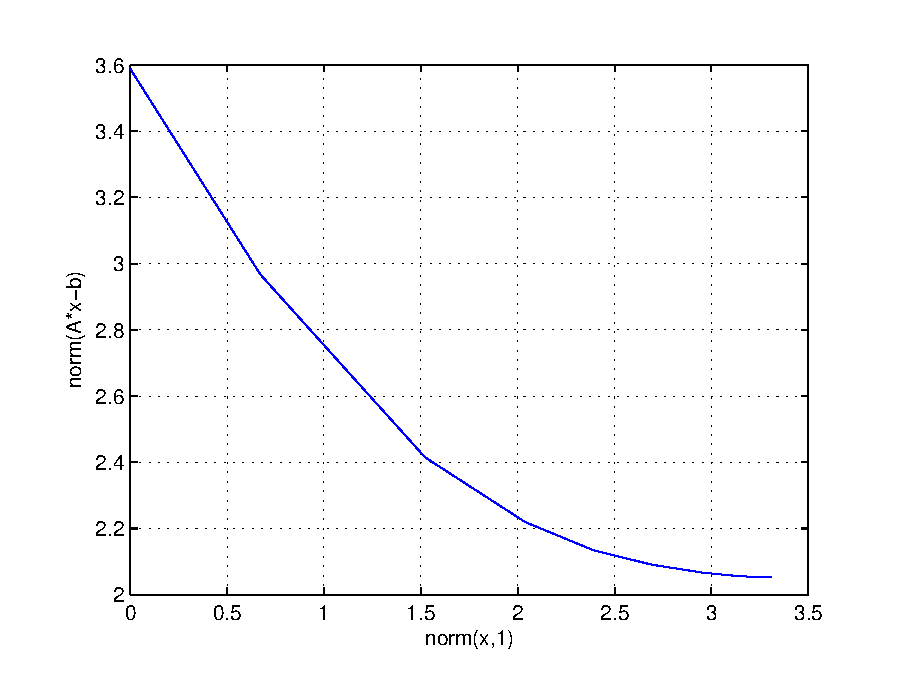
\includegraphics[width=4.5in]{tradeoff.eps}
\end{center}
~\\[-48pt]
\caption{An example tradeoff curve from the \texttt{quickstart} demo, lines \ref{code:tradeoffbeg}-\ref{code:tradeoffend}.}
\label{fig:tradeoff}
\end{figure}

Line~\ref{code:tradeoff} of this code segment illustrates one of the
construction rules to be discussed in \S\ref{sec:rules} below. A basic
principle of convex analysis is that a function known
to be convex can be multiplied by a nonnegative scalar,
or added to another function known to be convex, and the result
is then known to be convex. \cvx recognizes such combinations and allows
them to be used anywhere a simple convex function can be---such as an objective
function to be minimized, or on the appropriate side of an inequality
constraint. So in our example, the expression
\begin{code}
	norm(A*x-b)+gamma(k)*norm(x,1)
\end{code}
on line~\ref{code:tradeoff}
is recognized as convex by \cvx, as long as \verb@gamma(k)@
is positive or zero. If \verb@gamma(k)@ were negative, then
this expression becomes the sum of a convex term and a concave
term, which causes \cvx
to generate the following error:
\begin{code}
??? Error using ==> cvx.plus
Disciplined convex programming error:
Addition of convex and concave terms is forbidden.
\end{code}

\section{The basics}

\subsection{Data types for variables}

As mentioned above, all variables must be declared using the \verb@variable@
command (or the \verb@variables@ command; see below) before they can be
used in constraints or objective functions. 

Variables can be real or complex; and scalar, vector,
matrix, or $n$-dimensional arrays. In addition, matrices can have \emph{structure}
as well, such as symmetry or bandedness. The structure of a variable
is given by supplying a list of descriptive keywords after the name
and size of the variable.
For example, the code segment
\begin{code}
	variable w(50) complex;
	variable X(20,10);
	variable Y(50,50) symmetric;
	variable Z(100,100) hermitian toeplitz;
\end{code}
(inside a \cvx specification) declares that \verb@w@ is a complex
$50$-element vector, \verb@X@ is
a real $20 \times 10$ matrix optimization variable, \verb@Y@ is
a real $50 \times 50$ symmetric matrix optimization variable,
and \verb@Z@ is a complex $100 \times 100$ Hermitian matrix variable.
It is actually possible for the structure keywords to be applied to
$n$-dimensional arrays as well:
each 2-dimensional ``slice'' of the array
is given the stated structure. The list of possible structure
keywords are:
\begin{center}
\verb@banded(lb,ub)@\ \ \ \verb@complex@\ \ \ \verb@diagonal@\ \ \ \verb@hankel@\ \ \ \verb@hermitian@\ \ \ 
\verb@lower_bidiagonal@\ \ \ \verb@lower_hessenberg@\ \ \ \verb@lower_triangular@\ \ \ \verb@scaled_identity@\ \ \ 
\verb@skew_symmetric@\ \ \ \verb@symmetric@\ \ \ \verb@toeplitz@\ \ \ \verb@tridiagonal@\ \ \ 
\verb@upper_bidiagonal@\ \ \ \verb@upper_hankel@\ \ \ \verb@upper_hessenberg@\ \ \ \verb@upper_triangular@\ \ \ 
\end{center}
With a couple of exceptions, the structure keywords are self-explanatory:
\begin{itemize}
\item \verb@banded(lb,ub)@: the matrix is banded with a lower bandwidth \verb@lb@
and an upper bandwidth \verb@ub@. If both \verb@lb@ and \verb@ub@ are zero, then a 
diagonal matrix results. \verb@ub@ can be omitted, in which case it is set equal to \verb@lb@.
For example, \verb@banded(1,1)@ (or \verb@banded(1)@) is a tridiagonal matrix.
\item \verb@scaled_identity@: the matrix is a (variable) multiple of the identity matrix; that is,
it is diagonal and Toeplitz.
\item \verb@upper_hankel@, \verb@hankel@: An \verb@upper_hankel@ matrix is zero below
the antidiagonal; a \verb@hankel@ matrix is not (necessarily).
\end{itemize}
When multiple keywords are supplied, the resulting matrix structure is
determined by intersection; if the keywords conflict, then an error will result.

A \verb@variable@ statement can be used to declare only a single
variable, which can be a bit inconvenient if you have a lot of variables
to declare. For this reason, the statement \verb@variables@ statement
is provided which allows you to declare multiple variables; \ie,
\begin{code}
	variables x1 x2 x3 y1(10) y2(10,10,10);
\end{code}
The one limitation of the \verb@variables@ command is that it cannot
declare complex or structured arrays (\eg, \verb@symmetric@,
\emph{etc.}). Those must be declared
one at a time, using the singular \verb@variable@ command.

\subsection{Objective functions}

Declaring an objective function requires
the use of the \verb@minimize@ or \verb@maximize@ function, as
appropriate.  The objective function in a call to \verb@minimize@ 
must be convex; the objective function in a call to \verb@maximize@
must be concave. At most one objective function may be declared in a 
given \cvx specification, and the objective function must have a
scalar value. (For the only exception to this rule, see the 
section on defining new functions in \S\ref{s-new-fcts}).

If no objective function is specified, the problem is interpreted
as a feasibility problem, which is the same as performing a minimization
with the objective function set to zero. In this case, \verb@cvx_optval@
is either \verb@0@, if a feasible point is found, or
\verb@+Inf@, if the constraints are not feasible.

\subsection{Constraints}

The following constraint types are supported in \cvx:
\begin{itemize}
\item Equality \verb@==@ constraints, where both the left- and right-hand
sides are affine functions of the optimization variables.
\item Less-than \verb@<=@, \verb@<@ inequality constraints, where the left-hand
expression is convex, and the right-hand expression is concave.
\item Greater-than \verb@>=@, \verb@>@ constraints, where the left-hand
expression is concave, and the right-hand expression is convex.
In \cvx, \verb@<@ is the same as \verb@<=@, but we encourage you to
use the longer form \verb@<=@, since it is mathematically correct.
\end{itemize}

These equality and inequality operators work for arrays.
When both sides of the constraint are arrays of the same size,
the constraint is imposed elementwise.  If \verb@a@ and \verb@b@
are $m \times n$ matrices, for example, then \verb@a<=b@
is interpreted by \cvx as $mn$ (scalar) inequalities, \ie,
each entry of \verb@a@ must be less than or equal to
the corresponding entry of \verb@b@.
\cvx also handles equalities and inequalities where one side is 
a scalar and the other is an array.  This is interpreted as a
constraint for each element of the array, with the (same) scalar
appearing on the other side.
As an example, if \verb@a@ is an $m\times n$ matrix, then \verb@a>=0@ 
is interpreted as $mn$ inequalities: each element of the matrix
must be nonnegative.

Note also the important distinction between \verb@=@, which is an 
assignment, and \verb@==@, which imposes an equality constraint
(inside a \cvx specification).
Also note that the non-equality operator \verb@~=@ may \emph{not}
be used in a constraint, because it is rarely convex.
Inequalities cannot be used if either side is complex.

\cvx also supports a \emph{set membership} constraint; 
see \S\ref{sec:sets}.

\subsection{Functions}

The base \cvx function library
includes a variety of convex, concave, and affine functions
which accept \cvx variables or expressions as arguments.
Many are common Matlab functions
such as \verb@sum@, \verb@trace@, \verb@diag@, \verb@sqrt@,
\verb@max@, and \verb@min@,
re-implemented as needed to support \cvx; others are new
functions not found in Matlab.
A complete list of the functions in the base library 
can be found in \S\ref{s-functions}.
It's also possible to add your own new functions;
see \S\ref{s-new-fcts}.

An example of a function in the base library is
\verb@quad_over_lin@, which represents the
quadratic-over-linear function, defined as $f(x,y)=x^Tx/y$,
with domain $\R^n \times \R_{++}$, \ie,
$x$ is an arbitrary vector in $\R^n$, and $y$ is a positive
scalar.  (There is a version of this function that accepts
complex $x$, but we'll consider real $x$ to keep things simple.)
The quadratic-over-linear function is convex in 
$x$ and $y$, and so can be 
used as an objective, in an appropriate constraint, or in a 
more complicated expression.
We can, for example, minimize the quadratic-over-linear
function of $(Ax-b,c^Tx+d)$ using
\begin{code}
	minimize( quad_over_lin( A*x-b, c'*x+d ) );
\end{code}
inside a \cvx specification,
assuming \verb@x@ is a vector optimization variable,
\verb@A@ is a matrix, \verb@b@
and \verb@c@ are vectors, and \verb@d@ is a scalar.
\cvx recognizes this objective expression as a convex 
function, since it is
the composition of a convex function (the quadratic-over-linear
function) with an affine function.
You can also use the function \verb@quad_over_lin@ \emph{outside}
a \cvx specification.   In this case, it just computes its (numerical)
value, given (numerical) arguments.

\subsection{Sets}
\label{sec:sets}

\cvx supports the definition and use of convex sets.
The base library includes the cone of 
positive semidefinite $n \times n$ matrices,
the second-order or Lorentz cone, and various norm balls.
A complete list of sets supplied in the base library is given in 
\S\ref{s-functions}.

Unfortunately, the Matlab language does not have a 
set membership operator, such as \verb@x in S@, to denote $x \in S$.  
So in \cvx, we use a slightly different syntax to require
that an expression is in a set.
To represent a set we use a \emph{function} that returns
an unnamed variable that is required to be in the set.
Consider, for example, $\symm^n_+$, the cone of 
positive semidefinite $n \times n$ matrices.
In \cvx, we represent this by the function \verb@semidefinite(n)@,
which returns an unnamed new variable, that is constrained to be
positive semidefinite.
To require that the matrix expression \verb@X@ 
be positive semidefinite, we use the syntax \verb@X == semidefinite(n)@.
The literal meaning of this is that \verb@X@ is constrained to be 
equal to some unnamed variable, which is required to be 
an $n \times n$ symmetric positive semidefinite matrix. 
This is, of course, equivalent to saying that \verb@X@ must be
symmetric positive semidefinite.

As an example, consider the constraint
that a (matrix) variable \verb@X@ is a correlation
matrix, \ie, it is symmetric, has unit diagonal elements, and 
is positive semidefinite.  In \cvx we can declare such a variable
and constraints using
\begin{code}
	variable X(n,n) symmetric;
	X == semidefinite(n);
	diag(X) == ones(n,1);
\end{code}
The second line here imposes the constraint that \verb@X@
be positive semidefinite.
(You can read `\verb@==@' here as `is', so the second line can be 
read as `\verb@X@ is positive semidefinite'.)
The lefthand side of the third line
is a vector containing the diagonal elements of \verb@X@, whose 
elements we require to be equal to one. Incidentally, Matlab
allows us to simplify the third line to
\begin{code}
	diag(X) == 1;
\end{code}
because Matlab accepts comparisons between arrays and scalars
by comparing each element of the array independently with the scalar.

Sets can be combined in affine expressions, and we can constrain
an affine expression to be in a convex set.
For example, we can impose constraints of the form
\begin{code}
	A*X*A'-X == B*semidefinite(n)*B';
\end{code}
where \verb@X@ is an $n \times n$ symmetric variable matrix,
and \verb@A@ and \verb@B@ are $n \times n$  constant matrices.
This constraint requires that $AXA^T-X=BYB^T$, 
for some $Y \in \symm^n_+$.

\cvx also supports sets whose elements are ordered
lists of quantities.  As an example, consider the second-order or 
Lorentz cone,
\begin{equation}
	\lorentz^m = \Condset{ (x,y) \in \R^m\times\R }{ \| x \|_2 \leq y } = \epi \|\cdot\|_2,
\end{equation}
where $\epi$ denotes the epigraph of a function.
An element of $\lorentz^m$ is an ordered list, with two elements:
the first is an $m$-vector, and the second is a scalar.
We can use this cone to express the simple least-squares problem 
from \S\ref{sec:leastsquares} (in a fairly complicated way)
as follows:
\begin{equation}
	\begin{array}{ll}
		\text{minimize}   & y \\
		\text{subject to} & ( A x - b, y ) \in \lorentz^m.
	\end{array}
\end{equation}
\cvx uses Matlab's cell array facility to mimic this notation:
\begin{code}
	cvx_begin
	    variables x(n) y;
	    minimize( y );
	    subject to
	        { A*x-b, y } == lorentz(m);
	cvx_end
\end{code}
The function call \verb@lorentz(m)@ returns
an unnamed variable (\ie, a pair consisting of a vector and a 
scalar variable),
constrained to lie in the Lorentz cone of length \verb@m@. 
So the constraint in this
specification requires that the pair \verb@A*x-b@, \verb@y@, together, 
lie in the appropriately-sized Lorentz cone.

\cvx also provides a function \verb@in(x,S)@ as an alternative
to the set membership constraint syntax \verb@x==S()@.
For example, the lines
\begin{code}
	X == semidefinte(n);
	{ x, y } == lorentz( n );
\end{code}
can be rewritten
\begin{code}
	in( X, semidefinite(n) );
	in( { x, y }, lorentz( n ) );
\end{code}

\subsection{Dual variables}
When a disciplined convex program is solved, the associated 
\emph{dual problem} is also solved.
(In this context, the original problem is called the \emph{primal
problem}.)
The optimal dual variables, each of which is associated with a 
constraint in the original problem,
give valuable information about the original problem,
such as the sensitivities with respect to perturbing the constraints
\cite[Ch.5]{BV:04}.
To get access to the optimal dual variables in \cvx, you 
simply declare them, and associate them with the constraints.
Consider, for example, the LP
\[
\begin{array}{llcll}
\mbox{minimize} & c^Tx \\
\mbox{subject to} & Ax \preceq b
\end{array}
\]
with variable $x$, and $m$ linear inequality constraints.
The dual of this problem is
\[
\begin{array}{llcll}
\mbox{maximize} & b^T \lambda \\
\mbox{subject to} & A^T \lambda = c \\ & \lambda \succeq 0
\end{array}
\]
The dual variable $\lambda$ is associated with the inequality
constraint $Ax\preceq b$. To represent this association in \cvx,
we use the following syntax:
\begin{code}
	n = size(A,2);
	cvx_begin
	    variable x(n);
	    dual variable y;
	    minimize( c' * x );
	    subject to
	        y : A * x <= b;
	cvx_end
\end{code}	
The line 
\begin{code}
	dual variable y
\end{code}
tells \cvx that \verb@y@ will
represent a dual variable; and the line 
\begin{code}
	y : A * x <= b;
\end{code}
assigns \verb@y@ to the given inequality constraint. Notice how the
colon \verb@:@ operator is being used in a different manner than 
Matlab usually intends, which is to construct numeric sequences
like \verb@1:10@. This new behavior is in effect only
when a dual variable is present, so there should be no confusion 
or conflict.
The dimensions of dual variables are not specified 
when they are declared; they are
automatically determined from the constraints to which they 
are assigned.
For example, if $m=20$, \verb@y@ at the Matlab command prompt 
immediately before \verb@cvx_end@ yields
\begin{code}
y =
    cvx dual variable (20x1 vector)
\end{code}
After the \verb@cvx_end@ statement is processed, and assuming the
optimization was sucessful, \cvx assigns numerical values to
\verb@x@ and \verb@y@ (optimal primal and dual variable values,
respectively).

If $x$ and $y$ are primal and dual optimal variables for this LP,
they must satisfy $y_i(b-Ax)_i=0$, the so-called
\emph{complementary slackness conditions}.
You can check this in Matlab with the line
\begin{code}
	y .* (b-A*x)
\end{code}
which prints out the products of the entries of \verb@y@ and 
\verb@b-A*x@, which should be nearly zero.
This line must be executed \emph{after} the \verb@cvx_end@ command
(which assigns numerical values to \verb@x@ and \verb@y@); it will
generate an error if it is executed inside the \cvx specification,
where \verb@y@ and \verb@b-A*x@ are still just abstract expressions.

\section{The DCP ruleset}
\label{sec:rules}

As mentioned previously, \cvx enforces the conventions dictated by the
disciplined convex programming ruleset, or \emph{DCP ruleset} for short.
\cvx will issue an error message whenever it encounters a violation of any
one of the rules; hence it is important to understand
them before beginning to build models. Thankfully, the rules are drawn
from basic principles of convex analysis, and are easy to learn---especially
if you already construct convex programs regularly.

The DCP ruleset is a set of sufficient, but not necessary, conditions
for convexity. So it is possible to construct expressions that violate
the ruleset but are in fact convex. 
Indeed, it is not difficult to do so;
consider the well-known (and useful) entropy function,
\begin{code}
	- sum( x .* log( x ) )
\end{code}
This expression is easily verified to be concave over the values of \verb@x@ for which it is defined. But \cvx
rejects it as written, because it violates the 
no-product rule described in \S\ref{sec:noproduct}. 
Problems involving entropy, however, can be solved, by explicitly
using the entropy function, 
\begin{code}
	entropy( x )
\end{code}
which is in the base \cvx library, and thus recognized as 
concave by \cvx.
(The first version of \cvx, however, does not yet support the 
entropy function.)
If a convex (or concave) function is not recognized as
convex or concave by \cvx, it can be added as a new atom;
see \S\ref{s-new-fcts}.

At first, these restrictions may seem inconvenient,
especially to those accustomed to the more permissive nature of 
more traditional modeling frameworks.
We hope you will find that the rules are, in fact, not 
particularly restrictive
in practice; and certainly that they are a small price to pay 
for the considerable benefits they allow: automatic convexity 
verification, automatic
conversion to solvable form, and full support for nonsmooth functions. 

\subsection{Top-level rules}

\cvx currently allows three different types of disciplined convex programs:
\begin{itemize}
\item A \emph{minimization problem}, consisting of a convex objective function
and zero or more convex constraints.
\item A \emph{maximization problem}, consisting of a concave objective function
and zero or more concave constraints.
\item A \emph{feasibility problem}, consisting of one or more convex constraints.
\end{itemize}
Convexity is enforced for each constraint \emph{individually}, so it is not
sufficient for the intersection of the constraints to be convex. For example, the set
\begin{equation*}
	\Condset{ x\in \R }{ x^2 \geq 1, ~ x \geq 0 }
\end{equation*}
is convex (indeed, it is just the interval $[1,\infty)$), but its description
includes a nonconvex constraint $x^2 \geq 1$.

\subsection{Constraints}

Three types of constraints may be specified in disciplined convex programs:
\begin{itemize}
\item An \emph{equality constraint} \verb@==@ where both sides are affine expressions.
\item A \emph{less-than inequality constraint} \verb@<=@, \verb@<@ 
where the left side is convex and the right side is concave.
\item A \emph{greater-than inequality constraint} \verb@>=@, \verb@>@ 
where the left side is concave and the right side is convex.
\end{itemize}
Deliberately omitted from this list are \emph{non}-equality constraints; \ie,
constraints using the \verb@~=@ ($\neq$) operator. This is because, in general,
such constraints are not convex.

As discussed in \S\ref{sec:sets} above, \cvx enforces set 
membership constraints (\eg, $x\in S$) using
equality constraints. 
The rule that both sides of an equality constraint
must be affine applies to set membership constraints as well. 
In fact, the returned value of set atoms like 
\verb@semidefinite()@ and \verb@lorentz()@ is affine,
so it is sufficient to simply verify the remaining portion
of the set membership constraint. For composite values like
\verb@{ x, y }@, each element must be affine.

In this alpha version, 
strict inequalities \verb@<@, \verb@>@ are interpreted
identically to non-strict inequalities \verb@>=@, \verb@<=@. 
Eventually \cvx will flag strict inequalities so that they 
can be verified after the optimization is carried out.

\subsection{Expression rules}
\label{sec:noproduct}

So far, the rules as stated are not particularly restrictive, 
in that all convex programs (disciplined or otherwise) 
must adhere to them.
What distinguishes disciplined convex programming from more general
convex programming are the rules governing
the construction of the expressions used in objective functions and
constraints.

In disciplined convex programming, an expression is categorized by
its \emph{curvature}, which is either 
\emph{constant}, \emph{affine}, \emph{convex}, or \emph{concave}.
Disciplined convex programming determines curvature by recursively
applying the following rules:
\begin{itemize}
\item A valid constant is a MATLAB expression that evaluates
to a finite numeric value.
\item A valid affine expression is
\begin{itemize}
\item a constant expression;
\item a declared variable;
\item the sum of two or more affine expressions;
\item the difference between two affine expressions; or
\item the product of an affine expression and a constant.
\end{itemize}
\item A valid convex expression is
\begin{itemize}
\item a constant or affine expression;
\item a valid call to a convex function in the atom library;
\item a convex scalar quadratic form (\S\ref{sec:quadforms});
\item the sum of two or more convex expressions;
\item the difference between a convex expression and a concave expression;
\item the product of a convex expression and a nonnegative constant;
\item the product of a concave expression and a nonpositive constant; or
\item the negation of a concave expression.
\end{itemize}
\item A valid concave expression is
\begin{itemize}
\item a constant or affine expression;
\item a valid call to a concave function in the atom library;
\item a concave scalar quadratic form (\S\ref{sec:quadforms});
\item the sum of two or more concave expressions;
\item the difference between a concave expression and a convex expression;
\item the product of a concave expression and a nonnegative constant; 
\item the product of a convex expression and a nonpositive constant; or
\item the negation of a convex expression.
\end{itemize}
\end{itemize}
%In all of the above rules, it is assumed that the expressions are
%well-posed, in both a mathematical sense and according to MATLAB's
%own syntax rules. 
If an expression cannot be categorized by this ruleset, then it is 
rejected by \cvx (even if the expression is, in fact, convex).
For matrix and array expressions, these rules
are applied on an elementwise basis.
We also note that the set of rules listed above is redundant;
there are much smaller, equivalent sets of rules.

%While this list may seem long, it is for the most part an enumeration of basic
%rules of convex analysis for combining convex, concave, and affine forms: sums,
%multiplication by scalars, and so forth. 
These expression rules forbid \emph{products}
between nonconstant expressions, 
with the exception of scalar quadratic forms 
(see \S\ref{sec:quadforms} below).
We call this the \emph{no-product rule}.
These expression rules also forbid the use of 
nonconstant expressions as either the argument or exponent of a 
power expression (\verb@x ^ y@).

\subsection{Functions}

Because functions in the \cvx atom library are created in the 
Matlab language,
they differ in certain ways from functions described in a 
formal mathematical sense,
so let us address these differences here.

In disciplined convex programming, functions are categorized by their
curvature (\emph{constant}, \emph{affine},
\emph{convex}, or \emph{concave}) as well as their
\emph{monotonicity}
%\footnote{Strict monotonicity is not relevant to the DCP ruleset.}
(\emph{nondecreasing}, \emph{nonincreasing}, or \emph{nonmonotonic}).
Curvature determines the conditions
under which they can appear as in expressions according to the
expression rules given in \S\ref{sec:noproduct} above.
Monotonicity determines
how they can be used in function  compositions, 
as we shall see in \S\ref{sec:compositions} below.

For functions with only one argument, the categorization is 
straightforward.  As examples, we have:
\begin{center}
\begin{tabular}{lll}
	\verb@sum( x )@ & $\sum_i x_i$ & affine, nondecreasing \\
	\verb@abs( x )@ & $|x|$ & convex, nonmonotonic \\
	\verb@log( x )@ & $\log x$ & concave, nondecreasing
\end{tabular}
\end{center}
Convexity and monotonicity are always determined in an 
extended-valued sense.
For example, when its argument is a nonconstant
\cvx expression, Matlab's square root function \verb@sqrt( x )@ is
interpreted as follows:
\begin{center}
\begin{tabular}{lll}
	\verb@sqrt( x )@ & $\Cases{\sqrt{x}&x\geq 0\\-\infty&x<0}$ & concave, nondecreasing \\
\end{tabular}
\end{center}
(This intepretation has the effect of constraining the argument \verb@x@
to be nonnegative.) Furthermore, \cvx does \emph{not} consider a function to be
convex or concave if it is so only over a portion of its domain. 
For example, consider the function
\begin{center}
\begin{tabular}{lll}
	\verb@1/x@ & $1/x~~(x\neq 0)$ & not convex/concave/affine, nonomonotonic
\end{tabular}
\end{center}
This function is convex if its argument is positive, and
concave if its argument is negative.  Over its whole domain, though,
it is neither convex nor concave;
and in \cvx, of course, it is not recognized as either convex or 
concave.
However, the function
\begin{center}
\begin{tabular}{lll}
	\verb@inv_pos( x )@ & $\Cases{1/x &x>0\\+\infty&x\leq 0}$ & convex, nonincreasing
\end{tabular}
\end{center}
which is convex and nonincreasing,
has been included in the atom library,
so it can be used freely in constraints
and objective functions.

For functions that have multiple arguments, additional considerations must
be made. First of all, curvature is always considered \emph{jointly}, but montonicity
can be considered on an argument-by-argument basis. For example,
\begin{center}
\begin{tabular}{lll}
	\verb@quad_over_lin( x, y )@ & $\Cases{|x|^2/y&y> 0\\+\infty&y\leq 0}$ & concave, nonincreasing in \verb@y@
\end{tabular}
\end{center}
is jointly convex in both arguments, but it is monotonic 
only in its second argument.

In addition, some functions are convex, concave, or affine only for 
a \emph{subset} of its arguments. For example, the function
\begin{center}
\begin{tabular}{lll}
	\verb@norm( x, p )@ & $\|x\|_p~~(1<p<+\infty)$ & convex, nonmonotonic
\end{tabular}
\end{center}
is convex only in its first argument. Whenever this function is used
in a \cvx specification, then, the remaining
arguments must be constant, or \cvx will issue an error message. Such arguments
correspond to a function's parameters in a mathematical terminology; \eg,
\begin{equation*}
	f_p(x):\R^n\rightarrow\R, \quad f_p(x) \triangleq \|x\|
\end{equation*}
So it seems fitting that we should refer to such arguments as \emph{parameters}
in this context as well. Henceforth, whenever we speak of a \cvx function
as being convex, concave, or affine, we will assume that its parameters are
known and have been given appropriate, constant values.

\subsection{Compositions}
\label{sec:compositions}

A basic rule of convex analysis is that convexity is closed under 
composition with an affine mapping. 
This is part of the DCP ruleset as well:
\begin{itemize}
\item A convex, concave, or affine function may accept as an argument
any affine expression (assuming it is of compatible size).
\end{itemize}
(The result is convex, concave, or affine, respectively.)
For example, consider the function \verb@square( x )@, which is provided
in the \cvx atom library. 
This function squares its argument; \ie, it computes
\verb@x.*x@. 
(For array arguments, it squares each element independently.)
It is in the \cvx atom library, and known to be convex, provided its
argument is real.  So if \verb@x@ is a real variable, then
\begin{code}
	square( x )
\end{code}
is accepted by \cvx as a convex expression---and, thanks to
the above rule, so is
\begin{code}
	square( A * x + b )
\end{code}
if \verb@A@ and \verb@b@ are constant matrices of compatible size.

DCP also allows nonlinear functions to be combined using more
sophisticated composition rules. 
The general
DCP rules that govern these compositions are as follows:
\begin{itemize}
\item If a function is convex and nondecreasing in a given argument,
then that argument may be convex.
\item If a function is convex and nonincreasing in a given argument,
then that argument may be concave.
\item If a function is concave and nondecreasing in a given argument,
then that argument may be concave.
\item If a function is concave and nonincreasing in a given argument,
then that argument may be convex.
\end{itemize}
(In each case, we assume that the argument is of compatible size.)
For more on composition rules, see \cite[\S3.2.4]{BV:04}.
In fact, with the exception of scalar quadratic expressions,
the entire DCP ruleset can be thought of as specific manifestations
of these four rules.

For example, the pointwise maximum of convex functions is convex, because
the maximum function is convex and nondecreasing.
Thus if \verb@x@ is a vector variable then 
\begin{code}
	max( abs( x ) )
\end{code}
obeys the first of the four composition rules and is therefore accepted
by \cvx. In fact, the infinity-norm function \verb@norm( x, Inf )@
is defined in exactly this manner. 
Affine functions must obey these composition rules as well; but because they
are both convex and concave, they prove a bit more flexible. So, for example, 
the expressions
\begin{code}
	sum( square( x ) )
	sum( sqrt( x ) )
\end{code}
are both valid nonlinear compositions in \cvx, according to the 
convex/nondecreasing and concave/nondecreasing rules, respectively.
(The first is recognized as convex and nondecreasing, and the second
is recognized as concave and nondecreasing.)

Let us consider a more complex example in depth. Suppose
\verb@x@ is a vector variable, and
\verb@A@, \verb@b@, and \verb@f@ are 
constants with appropriate dimensions.  \cvx recognizes the
expression
\begin{code}
sqrt(f'*x) + min(4,1.3-norm(A*x-b))
\end{code}
as concave. Consider, for example, the first term, \verb@sqrt(f'*x)@.
\cvx recognizes \verb@f'*x@ as affine, and it knows that a concave
increasing function of a concave function is concave, so it
concludes that \verb@sqrt(f'*x)@ is concave.
(Incidently, when \verb@sqrt@ is used inside a \cvx specification,
it adds the constraint that its argument must
be nonnegative.)
\cvx recognizes that \verb@-norm(A*x-b)@ is concave,
since it is the negative of a convex function;
and it knows that the minimum of two concave functions is concave,
so it concludes that the second term,  \verb@min(4,1.3-norm(A*x-b))@,
is also concave.  The whole expression is then recognized as concave,
since it is the sum of two concave functions.

As these composition rules are sufficient but not necessary,
some expressions which are obviously convex or concave will fail to
satisfy them. For example, if \verb@x@ is a vector variable, the
expression
\begin{code}
	sqrt( sum( square( x ) ) )
\end{code}
is rejected by \cvx, because there is no rule governing the composition
of a concave nondecreasing function with a convex function.
Of course, the workaround is simple in this case: use \verb@norm( x )@ function instead,
since \verb@norm@ is in the atom library and known by \cvx to be convex.

\subsection{Monotonicity in nonlinear compositions}

Monotonicity is a critical aspect of the rules for nonlinear compositions. 
This has some consequences that are not so obvious, as we shall demonstrate here
by example. Consider the expression
\begin{code}
	square( square( A * x + b ) )
\end{code}
where \verb@square( A * x + b )@ was defined in the previous section.
This expression effectively raises each element of \verb@A*x+b@ to the fourth
power, and it is clearly elementwise convex. But
\cvx will not recognize it as such, because a convex function of a convex
expression is \emph{not} necessarily convex: for example,
\begin{code}
	square( square( A * x + b ) - 1 )
\end{code}
is not convex. The problem is that \verb@square@ is not monotonic,
so the composition rules cannot be applied.

Examination of these examples reveals a key difference:
in the first, the argument to the outer \verb@square@ is nonnegative;
in the second, it is not. If \cvx had access to this information, it could
indeed conclude that the first composition is convex by applying a
modified form of the first nonlinear composition rule.
Alas, for now, \cvx does not have such access; so it cannot make
such conclusions.
It must instead require
that outer functions be \emph{globally} monotonic.

There are many ways to modify this example that it complies with the ruleset.
One is to recognize that a constraint such as
\begin{code}
	square( square( a * x + b ) ) <= 1
\end{code}
is equivalent to
\begin{code}
	square( a * x + b ) <= z
	square( z ) <= 1
\end{code}
where \verb@z@ is a new variable. The equivalency of this decomposition
is a direct consequence of the monotonicity of 
\verb@square@ when \verb@z@
is nonnegative. In fact, \cvx performs this decomposition itself for
those nonlinear compositions that it accepts.

Another approach is to use an alternate outer function 
\verb@square_pos@,
which we have included in the library to implement
the following function $f$:
\begin{equation*}
	f(x) \triangleq (\max\{x,0\})^2 = \Cases{ x^2 & x \geq 0 \\ 0 & x \leq 0 }
\end{equation*}
Obviously, \verb@square@ and \verb@square_pos@ coincide when their
inputs are nonnegative. But \verb@square_pos@ is globally nondecreasing, so it
can be used as the outer function in a nonlinear composition. Thus, the expression
\begin{code}
	square_pos( square( a * x + b ) )
\end{code}
is mathematically equivalent to the rejected version, but satisfies the DCP
ruleset and is therefore acceptable to \cvx.
This is the reason several functions in the \cvx atom library come in two
forms: the ``natural'' form, and one that is modified in such a way 
that it is monotonic, and can therefore 
be used in compositions. Other such ``monotonic extensions''
include \verb@sum_square_pos@ and \verb@quad_pos_over_lin@. If you are
implementing a new function yourself, you might wish to consider if
a monotonic extension of that function would be a useful addition as well.

Yet another approach is to use one of the above techniques within
a \emph{new} function, say \verb@power4@, that enables the original
expression to be rewritten
\begin{code}
	power4( A * x + b )
\end{code}
and new expressions can now take advantage of the effort.
In \S\ref{s-new-fcts}, we show how to accomplish this.

\subsection{Scalar quadratic forms}
\label{sec:quadforms}

In its original form described in \cite{Gra:04,GBY},
the DCP ruleset forbids even the use of simple
quadratic expressions such as \verb@x * x@ (assuming \verb@x@ is a variable).
For practical reasons, we have chosen to make an exception to the ruleset to 
allow for the recognition of certain specific quadratic forms that map
directly to certain convex quadratic functions (or their concave negatives)
in the \cvx atom library:
\begin{center}
	\begin{tabular}{ccc}
	\verb@square( x )@ & $\Longrightarrow$ & \verb@conj(x) .* x@ \\
	\verb@sum_square( y )@ & $\Longrightarrow$ & \verb@y' * y@ \\
	\verb@quad_form( A * x - b, Q )@ & $\Longrightarrow$ &  \verb@(A*x-b)'*Q*(Ax-b)@
	\end{tabular}
\end{center}
In other words, \cvx detects quadratic expressions
such as those on the right above, and determines whether or not they
are convex or concave; and if so, translates them to an equivalent
function call, such as those on the left above.

When we say ``single-term'' above, we mean either a single product of
affine expressions, or
a single squaring of an affine expression. That is, \cvx
verifies each quadratic term \emph{independently}, not collectively.
So, for example, given scalar variables \verb@x@ and \verb@y@,
the expression
\begin{code}
	x ^ 2 + 2 * x * y + y ^2
\end{code}
will cause an error in \cvx, because the second of the three terms
\verb@2 * x * y@, is not convex. But equivalent expressions
\begin{code}
	( x + y ) ^ 2
	( x + y ) * ( x + y )
\end{code}
will be accepted. \cvx actually completes the
square when it comes across a scalar quadratic form, so the form
need not be symmetric. For example,
if \verb@z@ is a vector variable, \verb@a@, \verb@b@ are constants,
and \verb@Q@ is positive definite, then
\begin{code}
	( z + a )' * Q * ( z + b )
\end{code}
will be recognized as convex. Once a quadratic form has been verified by \cvx,
it can be freely
used in any way that a normal convex or concave expression can be,
as described in \S\ref{sec:noproduct}.

The use of quadratic forms should actually be
of \emph{less} use in disciplined convex programming
than in a more traditional mathematical programming framework,
where a quadratic form is often a smooth subsitute 
for a non-smooth form that one truly wishes to use. In
\cvx, such substitutions are rarely necessary, because of its support
for nonsmooth functions. For example,
the constraint
\begin{code}
	sum( ( A * x - b ) .^ 2 ) <= 1
\end{code}
is equivalently represented using the Euclidean norm:
\begin{code}
	norm( A * x - b ) <= 1
\end{code}
With modern solvers, the second form can be represented using a second-order cone
constraint---so the second form may actually be more efficient. So we encourage
you to re-evaluate the use of quadratic forms in your models, in light of the
new capabilities afforded by disciplined convex programming.

\section{Expanding the \cvx atom library}

The restrictions imposed by the DCP ruleset imply that,
for a fixed atom library, the variety of constraints and objective 
functions that can be constructed is limited.
Thus in order to preserve generality in
disciplined convex programming, the atom library must be extensible.
\cvx allows
you to define new convex and concave functions, and new convex sets, 
that can be used in \cvx specifications. 
This can be accomplished in a number of
ways, which we describe in this section.

\subsection{Defining new functions via overloading}
\label{s-new-fcts}

The simplest method of constructing a new function is to use the 
standard function definition mechanism in Matlab, and to rely on
the overloaded operators to do the right thing when the function is
invoked inside a \cvx specification.

To illustrate this, we consider the \emph{deadzone} function,
defined as
\[
f(x) = \max \{ |x|-1, 0 \} =
\left\{ \begin{array}{ll}
0 & |x| \leq 1\\
x-1 & x > 1\\
1-x & x <-1
\end{array}\right.
\]
The deadzone function is convex in $x$.  

It's very straightforward to add this function to \cvx.   In a file
\verb@deadzone.m@ we put the following code:
\begin{code}
	function y = deadzone( x )
	y = max( abs( x ) - 1, 0 )
\end{code}
This is nothing but a standard Matlab function, and it works
outside of \cvx 
(\ie, when it arguments are numerical), and also inside
\cvx (when its arguments are expressions).
The reason it works inside a \cvx specification is that the operations
carried out all conform to the rules of DCP:
\verb@abs@ is recognized as a convex function; we can subtract 
a constant from it, and we can take the maximum of the result and 
\verb@0@, which yields a convex function.
Inside \cvx, we can use \verb@deadzone@ anywhere we can
use \verb@norm@, for example; 
\cvx knows that it is a convex function.

Now consider what happens if we replace \verb@max@ with \verb@min@
in our definition of the \verb@deadzone@ function.
(The function $\min \{ |x|-1, 0 \}$ is neither convex nor concave.)
The modified function will work \emph{outside}
a \cvx specification, happily computing and returning 
the \emph{number} $\min \{|x|-1,0\}$, given a \emph{numerical}
argument $x$.
But inside a \cvx specification, and invoked 
with a nonconstant argument,
the modified function won't work,
since we haven't followed the DCP composition rules.

This method of defining an ordinary function, and relying on
overloading of operators inside a \cvx specification,
works provided you make sure that that all the 
calculations carried out inside
the function satisfy the DCP composition rules.

\subsection{Defining new functions via incomplete specifications}

Suppose that $S\subset\R^n\times\R^m$ is a convex set and 
$g:(\R^n\times\R^m)\rightarrow(\R\cup+\infty)$ is a convex function.
Then convex analysis tells us that
\begin{equation}
	\label{eq:partial}
	f:\R^n\rightarrow(\R\cup+\infty), \quad f(x) \triangleq \inf\Condset{g(x,y)}{(x,y)\in S }
\end{equation}
is also a convex function. In effect, $f$
has been expressed in terms of a parameterized 
family of convex optimization problems, where $x$ is
the family parameter.
One special case should be very familar: if $n=1$ and
$g(x,y)\triangleq y$, then
\begin{equation}
	f(x) \triangleq \inf\Condset{y}{(x,y)\in S}
\end{equation}
gives the classic \emph{epigraph} representation of $f$; that is, $S=\epi f$.

A key feature of \cvx is the ability to define a convex
function in this very manner: that is, in terms of a 
parameterized family of disciplined convex programs. 
We call the underlying convex program in such cases
an \emph{incomplete specification}---so names because
the parameters (that is, the function inputs)
are unknown when the specification is
constructed. The concept of incomplete 
specifications can at first seem a bit complicated,
but it is quite powerful, allowing
\cvx to support a variety of functions that cannot be
employed in a traditional, derivative-based optimization framework.

Let us look at an example to see how this works.
Consider the unit-halfwidth Huber penalty function $h(x)$:
\begin{equation}
	h:\R\rightarrow\R, \quad h(x) \eqbydef \Cases{ x^2 & |x| \leq 1 \\ 2|x|-1 & |x| \geq 1 }
\end{equation}
The Huber penalty function cannot be used in an optimization algorithm
utilizing Newton's method,
because its Hessian is zero for $|x|\geq 1$. However,
it can be expressed in terms of the following family of convex QPs,
parameterized by $x$:
\begin{equation}
	\begin{array}{ll}
		\text{minimize}   & 2 v + w^2 \\
		\text{subject to} & | x | \leq v + w \\
		                  & w \leq 1
	\end{array}
\end{equation}
Specifically, the optimal value of the this QP is equal to the Huber
penlaty function.
We can implement the Huber penalty function in \cvx as follows:
\begin{code}
	function cvx_optval = huber( x )
	cvx_begin
	    variables w v;
	    minimize( w^2 + 2 * v );
	    subject to
	        abs( x ) <= w + v;
	        w <= 1;
	cvx_end
\end{code}
If \verb@huber@ is called with a numeric value of \verb@x@, then
upon reaching the \verb@cvx_end@ statement, \cvx will find a complete
specification, and solve the problem to compute the result.
\cvx places the optimal objective function value
into the variable \verb@cvx_optval@, and
function returns that value as its output.

What is most important, however, is that if \verb@huber@
is used within a \cvx specification, with an affine \cvx expression
for it argument, then \cvx will do the right thing.
In this case, the function \verb@huber@ will contain a special Matlab object that
represents the function call in constraints and objectives.
Thus \verb@huber@ can be used anywhere a traditional convex
function can be used, in constraints or objective functions,
in accordance with the DCP ruleset.

There is a corresponding development for concave functions as well.
Given the set
$S$ above and a concave function
$\bar{g}:(\R^n\times\R^m)\rightarrow(\R\cup+\infty)$ is
concave, the function
\begin{equation}
	\label{eq:partial2}
	\bar{f}:\R\rightarrow(\R\cup+\infty), \quad \bar{f}(x) \triangleq \sup\Condset{g(x,y)}{(x,y)\in S }
\end{equation}
is also a concave function.
If $\bar{g}(x,y)\triangleq y$, then
\begin{equation}
	\bar{f}(x) \triangleq \sup\Condset{y}{(x,y)\in S}
\end{equation}
gives the \emph{hypograph} representation of $\bar{f}$; that is, $S=\hypo f$.
In \cvx, a concave incomplete specification is simply one that
uses a \verb@maximize@ objective instead of a \verb@minimize@ objective;
and if properly constructed, it can be used anywhere a traditional
concave function can be used within a \cvx specification. 

For an example of a concave incomplete specification, consider the function
\begin{equation}
	f:\R^{n\times n}\rightarrow\R, \quad f(X) = \lambda_{\min}(X+X^T)
\end{equation}
Its hypograph can be represented using a single linear matrix inequality:
\begin{equation}
	\hypo f = \Condset{ (X,t) }{ f(X) \geq t } = \Condset{ (X,t) }{ X + X^T - t I \succeq 0 }
\end{equation}
So we can implement this function in \cvx as follows:
\begin{code}
	function cvx_optval = lambda_min_symm( X )
	n = size( X, 1 );
	cvx_begin
	    variable y;
	    maximize( y );
	    subject to
	        X + X' - y * eye( n ) == semidefinite( n );
	cvx_end
\end{code}
If a numeric value of \verb@X@ is supplied, this function will return
\verb@min(eig(X+X'))@ (to within numerical tolerances). However, this function
can also be used in \cvx constraints and objectives, just like any other concave
function in the atom library.

There are two practical issues that arise when defining functions
using incomplete specifications, both of which are illustrated well by
our \verb@huber@ example above. First of all, as written the function works
only with scalar values. To apply it to a vector requires that we iterate
through the elements in a \verb@for@ loop---a \emph{very} inefficient enterprise,
particularly in \cvx. A far better 
approach is to extend the \verb@huber@ function to handle vector inputs. This
is, in fact, rather simple to do: we simply create a \emph{multiobjective}
version of the problem:
\begin{code}
	function cvx_optval = huber( x )
	sx = size( x );
	cvx_begin
	    variables w( sx ) v( sx );
	    minimize( w .^ 2 + 2 * v );
	    subject to
	        abs( x ) <= w + v;
	        w <= 1;
	cvx_end
\end{code}
This version of \verb@huber@ will in effect create \verb@prod( sx )@ ``instances''
of the problem in parallel; and when used in a \cvx specification,
\cvx will do the right thing.

The second issue is that if the input to \verb@huber@ is numeric, then
direct computation is a far more efficient way to compute the result
than solving a convex program. (What is more, the multiobjective version
cannot be used with numeric inputs.) One solution is to place 
both versions in one file, with an appropriate test to select
the proper version to use:
\begin{code}
	function cvx_optval = huber( x )
	if isnumeric( x ),
	    xa   = abs( x );
	    flag = xa < 1;
	    cvx_optval = flag .* xa.^2 + (~flag) * (2*xa-1);
	else,
	    sx = size( x );
	    cvx_begin
	        variables w( sx ) v( sx );
	        minimize( w .^ 2 + 2 * v );
	        subject to
	            abs( x ) <= w + v;
	            w <= 1;
	    cvx_end
	end
\end{code}
Alternatively, you can create two separate versions of the function, one 
for numeric input and one for \cvx expressions; and 
place the numeric version in a subdirectory called
\verb+@double+. Matlab will call the \verb+@double+ version only when its
arguments are numeric, and it will call your \cvx version in other cases.
This is the approach taken for the version of \verb@huber@ found in the \cvx
atom library.

One good way to learn more about using incomplete specifications is to
examine some of the examples already in the \cvx atom library. 
Good choices include \verb@huber@, \verb@inv_pos@, \verb@lambda_min@,
\verb@lambda_max@, \verb@matrix_frac@, \verb@quad_over_lin@,
\verb@sum_largest@, and others. Some are
a bit difficult to read because of diagnostic or error-checking code,
but these are relatively simple.

%\subsection{New differentiable atoms}
%Future versions of \cvx will support smooth functions as well.
%mention new atoms possible (see \S XXX). must provide fct value,
%gradient, and hessian.

\subsection{Defining new sets}

This version of \cvx does not support user-defined sets,
since we haven't yet settled on the best syntax.
This support will be added soon.

\iffalse
We can define new sets in \cvx in three basic ways, two of which
are supported in this first release.
The simplest is to use expressions and overloading, and the usual
function construction in Matlab.  But since only affine operations
can be applied to sets, this method cannot generate very 
interesting sets. 

The second method is analogous to specifying a convex or concave
function via an incomplete \cvx problem specification.
We describe a set by some constraints, given in \cvx form.
As an example, let's define a new set \verb@simplex(n)@, which is the
unit simplex in $\R^n$, defined as $\{x \in \R^n \;|\; 
x \succeq 0,~\ones^T x\leq 1 \}$.
To define this set, we create a file \verb@simplex.m@ containing
the following:
\begin{code}
function cvx_optval = simplex( n )
cvx_begin_set
variable x(n)
sum( x ) <= 1
x >= 0
cvx_end
\end{code}
We can now use this set in \cvx specifications.  For example, 
the line
\begin{code}
	A*x+b == simplex (size(A,1)) 
\end{code}
requires that $Ax+b$ must lie in the simplex of appropriate
dimension.
(Here we assume that \verb@x@ is a vector variable or affine
expression, and that \verb@A@ and \verb@b@ are a constant
matrix and vector, respectively, all of appropriate dimensions.

The one interesting twist is the use of the command 
\verb@cvx_begin_set@, instead of the usual \verb@cvx_begin@.
We can't use \verb@cvx_begin@ here, since the \cvx specification
above is \emph{complete}; it is interpreted as a feasibility problem.
If we used \verb@cvx_begin@ in this function, then when we call it,
\cvx forms the feasibility problem, discovers that it is complete,
and therefore solves it when it reaches the \verb@cvx_end@ command.
This problem is obivously feasible, so \verb@cvx_optval@ is \verb@0@,
so our function would simply always return \verb@0@.

XXX is it \verb@cvx_optval@ we want returned or \verb@x@?

The third method for defining a general convex set, with nonempty
interior, is to provide a barrier function (and its first and 
second derivatives) for the set.
This is not supported in the current version.
\fi

\newpage
\appendix

\section{Installing \cvx}
\label{s-installing}

The basic system requirements for running \cvx are Matlab 6.0 or later,
on any platform that supports SeDuMi 1.1R2 \cite{SeDuMi}. A copy of SeDuMi
has been included with \cvx.
The SeDuMi MEX files, and the lone \cvx MEX file, have been precompiled
for Windows, Linux, and Solaris 8, and we are able
to test them on the following specific platform combinations:
\begin{itemize}
\item Windows: MATLAB 6.1, 6.5.2, and 7.0.4.
\item Linux: MATLAB 6.5.1, 7.0.0, and 7.0.4.
\item Solaris 8: MATLAB 6.5.1 and 7.0.0.
\end{itemize}
If any of these combinations matches your own, then simply follow the directions in
\S\ref{sec:winlin} below to install \cvx, and you should be able to
proceed without difficulty.
For other platforms, please see the instructions in \S\ref{sec:othersys}.

If your platform combination differs only slightly from these---say,
for example, you are running Matlab 7.0.0 
on Windows---then the instructions in \S\ref{sec:winlin} \emph{should}
work, but we cannot be sure. We encourage
you to upgrade to at least upgrade to the latest minor version of
Matlab if at all possible; your license likely allows it.

If you have been running a previous version of \cvx, and you are installing
a new version, please do not simply unpack it on top of the old version. Instead,
remove the old version entirely, or move it out of the way---say, by renaming
the directory \verb@cvx@ to \verb@cvx.old@. Then follow the
directions as if you were installing \cvx for the first time.

\subsection{Precompiled platforms}
\label{sec:winlin}

Installing \cvx is simplest on Windows and Linux systems. If you are running Matlab
R13 (6.5), please note the additional instructions below:
\begin{enumerate}
\item Retrieve the latest version of cvx from \url{http://www.stanford.edu/~boyd/cvx}.
You can download the package as either a \verb@.zip@ file or a \verb@.tar.gz@ 
file.
\item Unpack the file anywhere you like; a directory called \verb@cvx@ will be created.
\item Start MATLAB.
\item Change the current directory to the location of \cvx.
For example, if you unpacked \verb@cvx.zip@ on your Windows machine into the
directory \verb@C:\Matlab\personal@, then you would type
\begin{code}
		cd C:\Matlab\personal\cvx
\end{code}
at the Matlab command prompt. Alternatively, if you unpacked \verb@cvx.tar.gz@
into the directory \verb@~/matlab@ on a Linux machine, then you would type
\begin{code}
		cd ~/matlab/cvx
\end{code}
at the Matlab command prompt.
\item Type the command
\begin{code}
		cvx_setup
\end{code}
at the Matlab prompt. This does two things: 
it sets the MATLAB search path so it can find all of the \cvx program files,
and it runs a simple test problem to verify the installation.
If all goes well, the command will output the line
\begin{code}
	No errors! cvx has been successfully installed.
\end{code}
(among others). If this message is not displayed, or any warnings or errors are generated,
then there is a problem with the \cvx installation. Try installing the package
again; and if that fails, send us a bug report and tell us about it.
\item If you plan to use \cvx regularly, you will need to save the current
MATLAB path for subsequent MATLAB sessions. Follow the instructions provided
by \verb@cvx_setup@ to accomplish that.
\end{enumerate}

\subsection{Other platforms}
\label{sec:othersys}

According to the SeDuMi web site, SeDuMi 1.1R2 will also run on MacOS X, AIX, and 
Solaris. If you wish to \cvx on these platforms, you will have
to compile SeDuMi's MEX files yourself. The installation thus proceeds as follows:
\begin{enumerate}
\item Install \cvx according to Steps 1-3 in \S\ref{sec:winlin}.
\item At the Matlab command prompt, \verb@cd@ to the directory \verb@sedumi@
within the \cvx installation, and execute the command 
\begin{code}
	install_sedumi
\end{code}
which will compile the MEX files.
\item Now complete steps 4-6 in \S\ref{sec:winlin} above.
\item It is likely that \verb@cvx_setup@ will warn you that it was unable to
      find the MEX file \verb@cvx_bcompress_mex@. To create it, \verb@cd@
      to the directory \verb@lib@ within the \cvx installation, and type
      the command
      \begin{code}
      		mex cvx_bcompress_mex.c
      \end{code}
      This assumes that you are properly set up to compile MEX files already;
      see your MATLAB documentation for more details.
\end{enumerate}
If you succced in compiling the MEX files for a new platform, please consider
sending them to us so that we may consider adding them to the master \cvx
distribution.

\emph{Important note:} If you are using Linux,
do \emph{not} run \verb@install_sedumi@. Doing so can result in 
errors that prevent SeDuMi and \cvx from running.

\subsection{About SeDuMi}

As stated above, 
the \cvx distribution includes a full copy of the SeDuMi package
in the directory \verb@cvx/sedumi@.
If you wish to use SeDuMi independently of \cvx, 
add that subdirectory to your Matlab path as well. 
If you already have SeDuMi installed on your system, you are free to remove
\verb@cvx/sedumi@ to save space; \cvx will detect the presence of your other
copy and use it instead. If you do this, it is important that
your version of SeDuMi coincides with the version used by \cvx (1.1R2).

\section{Operators, functions, and sets}
\label{s-functions}

\subsection{Basic operators and linear functions}

Matlab's standard arithmetic operations for
addition \verb@+@, subtraction \verb@-@, multiplication
\verb@*@ \verb@.*@, division \verb@/@ \verb@\@ \verb@./@
\verb@./@ \verb@.\@, and exponentiation \verb@^@ \verb@.^@
have been overloaded to work in \cvx whenever appropriate---that
is, whenever their use is consistent with both standard mathematical
and MATLAB conventions \emph{and} the DCP ruleset.
For example:
\begin{itemize}
\item Two \cvx expressions can be added together if they are of the same
      dimension (or one is scalar) and have the same curvature (\ie, 
      both are convex, concave, or affine).
\item A \cvx expression can be multiplied or divided by a scalar constant. If the
      constant is positive, the curvature is preserved; if it is negative,
      curvature is reversed.      
\item An affine, column vector \cvx expression can be multiplied by a constant matrix
      of appropriate dimensions; or it can be left-divided by a non-singular 
      constant matrix of appropriate dimension.
\end{itemize}
Numerious other combinations are possible, of course.
The use of the exponentiation operators \verb@^@ \verb@.^@ are limited
to instances that produce quadratic forms; so, for example, the exponent
must be 2.

Matlab's basic matrix manipulation and arithmetic
operations have been extended to work with
\cvx expressions as well, including:
\begin{itemize}
\item Concatenation: \verb@[ A, B ; C, D ]@
\item Indexing: \verb@x(n+1:end)@, \verb@X([3,4],:)@, \etc
\item Indexed assignment, including deletion: \verb@y(2:4) = 1@, \verb@Z(1:4,:) = []@, \etc
\item Transpose and conjugate transpose: \verb@Z.'@, \verb@y'@
\end{itemize}
A number of Matlab's basic functions have been extended to work with \verb@cvx@
expressions as well:
\begin{center}
\verb@conj@\ \ \ \verb@cumsum@\ \ \ \verb@diag@\ \ \ \verb@dot@\ \ \ \verb@fliplr@\ \ \ \verb@flipud@\ \ \ \verb@flipdim@\ \ \ \verb@horzcat@\ \ \ \
\verb@hankel@\ \ \ \verb@ipermute@\ \ \ \verb@kron@\ \ \ \verb@permute@\ \ \ \verb@repmat@\ \ \ \verb@reshape@\ \ \ \
\verb@rot90@\ \ \ \verb@sum@\ \ \ \verb@trace@\ \ \ \verb@tril@\ \ \ \verb@triu@\ \ \ \verb@toeplitz@\ \ \ \verb@vertcat@
\end{center}
Most should behave identically with \cvx expressions as they do with numeric expressions.
Those that perform some sort of summation, such as \verb@cumsum@, \verb@sum@, or
multiplication, such as \verb@dot@ or \verb@kron@, can
only be used in accordance with the disciplined convex programming rules. For example,
\verb@kron(X,Y)@ is valid only if either \verb@X@ or \verb@Y@ is constant; and 
\verb@trace(Z)@ is valid only if the elements along the diagonal have the same curvature.

\subsection{Standard Matlab nonlinear functions}
The following standard Matlab nonlinear functions 
are overloaded to work in \cvx:
\begin{itemize}
\item \verb@abs@, elementwise absolute value for real 
and complex arrays.
Convex.
\item \verb@max@, \verb@min@,
elementwise maximum and minimum, for real arrays only.
The 1, 2, and 3-argument syntaxes are all supported.
\verb@max@ is convex and increasing; \verb@min@ is concave and 
decreasing.
\item \verb@norm( x, 1 )@ and \verb@norm( x, Inf )@,
for real and complex vectors and matrices.
Convex.
\item \verb@norm( x )@ or \verb@norm( x, 2 )@, 
for real and complex vectors and matrices.
Convex.
\item \verb@norm( X, 'fro' )@, for real and complex matrices.
Convex.
\item \verb@sqrt@, elementwise squareroot, for real arrays only.
Adds constraint that entries are nonnegative.
Concave and increasing.
\end{itemize}

We note that in this version of \cvx, powers such as \verb@x^4@
or \verb@x^(1/2)@, are \emph{not} supported.

\subsection{New nonlinear functions}

The following functions are part of the base \cvx library.
These functions work both inside a \cvx specification,
and outside a \cvx specification (with numerical arguments).
\begin{itemize}
%\item \verb@geomean@, geometric mean,
%$\left( \prod_{k=1}^n x_k \right)^{1/n}$.  Inside a \cvx
%specification, adds constraint
%that arguments are all nonnegative.
%When evaluated outside a \cvx specification, returns $-\infty$
%if any $x_k$ is negative.
%Concave and increasing.
%\item XXX \verb@detroot@: $n$-th root of the determinant of a symmetric matrix:
%\begin{equation*}
	%g:\R^{n\times n}\rightarrow\R\cup-\infty, \quad
	%g(X) = \Cases{ (\det X)^{1/n} & X=X^T,~X\succeq 0 \\ -\infty & \text{otherwise} }
%\end{equation*}
\item \verb@huber(x)@, defined as $2|x|-1$ for $|x|\geq 1$,
and $x^2$ for $|x|<1$.  Convex.
\item \verb@inv_pos@, inverse of the positive portion, $1/\max\{x,0\}$.
Inside \cvx specification,
imposes constraint that its argument is positive.
Outside \cvx specificatiom, returns $+\infty$ if $x\leq 0$.
Convex and decreasing.
\item \verb@lambda_max@: maximum eigenvalue of a real symmetric 
or complex Hermitian matrix.
Inside \cvx, imposes constraint that its argument 
is symmetric (if real) or Hermitian (if complex).
Convex.
\item \verb@lambda_min@: minimum eigenvalue of a real symmetric 
or complex Hermitian matrix.
Inside \cvx, imposes constraint that its argument 
is symmetric (if real) or Hermitian (if complex).
Concave.
\item \verb@matrix_frac(x,Y)@: matrix fractional function,
$x^TY^{-1}x$.  In \cvx, imposes constraint that $Y$ is 
symmetric (or Hermitian) and positive definite; outside \cvx,
returns $+\infty$ unless $Y=Y^T\succ 0$.
Convex.  
%Note that \cvx will \emph{not} recognize \verb@x'*(Y\x)@ as convex.
\item \verb@norm_largest( x, k )@, for real and complex vectors.
Convex.
\item \verb@norms( x, p, dim )@ and \verb@norms( x, 'largest', k, dim )@.
Computes \emph{vector} norms along a specified dimension of a matrix
or N-d array. Useful for sum-of-norms and max-of-norms problems.
Convex.
\item \verb@pos@, $\max\{x,0\}$, for real $x$. 
Convex and increasing.
\item \verb@quad_form(x,P)@, $x^TPx$ for real $x$ and symmetric $P$,
and $x^HPx$ for complex $x$ and Hermitian $P$.
Convex in $x$ for $P$ constant and positive semidefinite;
concave in $x$ for $P$ constant and negative semidefinite.
This function is provided since \cvx will \emph{not}
recognize \verb@x'*P*x@ as convex (even when \verb@P@ is 
positive semidefinite).
\item \verb@quad_over_lin@, $x^Tx/y$ for $x \in \R^n$, $y >0$;
for $x \in \complex^n$, $y>0$: $x^*x/y$.  In \cvx specification,
adds constraint that $y>0$.  Outside \cvx specification,
returns $+\infty$ if $y\leq 0$.
Convex, and decreasing in $y$.
\item \verb@quad_pos_over_lin@: \verb@sum_square_pos( x ) / y@
for $x\in\R^n$, $y>0$.
Convex, increasing in $x$, and decreasing in $y$.
%XXX \item \verb@rel_diff@, Relative (fractional) difference between 
%two numbers, $\max\{x/y, y/x\} -1$.  Inside \cvx, imposes constraint
%that $x$ and $y$ are positive.  Outside \cvx, returns $+\infty$
%if $x \leq 0$ or $y\leq 0$. Convex.
\item \verb@sigma_max@: maximum singular value of real or 
complex matrix.  Same as \verb@norm@.  Convex.
\item \verb@square@: $x^2$ for $x \in \R$;
$|x|^2$ for $x \in \complex$.
Convex.
\item \verb@square_pos@: $\max\{x,0\}^2$ for $x\in\R$.
Convex and increasing.
\item \verb@sum_largest(x,k)@ sum of the largest $k$ values, for
real vector $x$.
Convex and increasing.
\item \verb@sum_smallest(x,k)@, sum of the smallest $k$ values,
\ie, \verb@-sum_smallest(-x,k)@.
Concave and decreasing.
\item \verb@sum_square@: \verb@sum( square( x ) )@. Convex.
\item \verb@sum_square_pos@: \verb@sum( square_pos( x ) )@; 
works only for real values. Convex and increasing.
\end{itemize}

\iffalse
Functions to be added when smooth function support is added: 
\begin{itemize}
\item \verb@exp@: $\exp$
\item \verb@log@: $\log$
\item \verb@log2@: $\log_2$
\item \verb@a^x@: $a^x$.  requires $a>0$.
\item \verb@x^a@: $x^a$.  requires $x>0$.
\item \verb@entropy@: entropy $-x \log x$
\item \verb@rel_entropy@: relative entropy
\item \verb@kl_div@: Kullback-Leibler divergence
\item \verb@log_sum_exp@: $\log(\sum_i \exp x_i)$
\item \verb@norm( x, p )@
\item \verb@log_det@
\item \verb@nth_root_det@
\item \verb@log_tsqr_minus_xsqr@: $\log (t^2-x^Tx)$
\item \verb@log_erf@: $\log \Phi$
\end{itemize}
\fi

\subsection{Sets}

\cvx currently supports the following sets; in each case, \verb@n@ is a positive
integer constant:
\begin{itemize}
\item \verb@nonnegative(n)@:
\begin{equation*}
	\reals^n_+ \eqbydef \Condset{x\in\Rn}{x_i\geq 0,~i=1,2,\dots,n}
\end{equation*}	
\item \verb@lorentz(n)@:
\begin{equation*}
\lorentz^n \eqbydef \Condset{(x,y)\in\R^n\times\R}{\|x\|_2\leq y}
\end{equation*}
\item \verb@rotated_lorentz(n)@: 
\begin{equation*}
\lorentz^n_r \eqbydef \Condset{(x,y,z)\in\R^n\times\R\times\R}{\|x\|_2\leq yz,~y,z\geq 0}
\end{equation*}
\item \verb@complex_lorentz(n):@ 
\begin{equation*}
\lorentz^n_c \eqbydef \Condset{(x,y)\in\complex^n\times\R}{\|x\|_2\leq y}
\end{equation*}
\item \verb@rotated_complex_lorentz(n)@: 
\begin{equation*}
\lorentz^n_{rc} \eqbydef \Condset{(x,y,z)\in\complex^n\times\R\times\R}{\|x\|_2\leq yz,~y,z\geq 0}
\end{equation*}
\item \verb@semidefinite(n):@ 
\begin{equation*}
\symm^n_+ \eqbydef \Condset{X\in\R^{n\times n}}{X=X^T,~X\succeq 0}
\end{equation*}
\item \verb@hermitian_semidefinite(n):@ 
\begin{equation*}
\herm^n_+ \eqbydef \Condset{Z\in\complex^{n\times n}}{Z=Z^H,~X\succeq 0}
\end{equation*}
\end{itemize}

\section{\cvx commands}

\begin{itemize}
\item \verb+cvx_problem+: typing this within a \cvx specification provides a summary
of the current problem. Note that this will contain a \emph{lot} of information
that you may not recognize---\cvx performs its conversion to canonical form
\emph{as the problem is entered}, generating extra temporary variables and
constraints in the process.
\item \verb+cvx_clear+: typing this resets the \cvx system, clearing any and all problems
from memory, but without erasing any of your numeric data.
This is useful if you make a mistake and need to start over.
\item \verb@cvx_quiet@: typing \verb@cvx_quiet(true)@ suppresses screen
output from the solver. Typing \verb@cvx_quiet(false)@ restores the screen
output. In each case, it returns a logical value representing the \emph{previous}
state of the quiet flag, so you can restore that state later if you wish.
\item \verb@cvx_pause@: typing \verb@cvx_pause(true)@ causes \cvx to pause and
wait for keyboard input before \emph{and} after the solver is called. Useful
primarily for demo purposes. Typing \verb@cvx_pause(false)@ resets the behavior.
In each case, it returns a logical value representing the \emph{previous} state
of the pause flag, so you can restore that state later if you wish.
\item \verb@cvx_where@: returns the directory where the \cvx distribution
has been installed---assuming that the Matlab path has been set to include
that distribution. Useful if you want to find certain helpful subdirectories,
such as \verb@doc@, \verb@examples@, \emph{etc.}
\end{itemize}

\section{\cvx status messages}
\label{sec:status}

After a complete \cvx specification has been entered and the \verb@cvx_end@ command 
issued, the solver is called to generate a numerical result. The solver can produce
one of five exit conditions, which are indicated by the value of the string variable
\verb@cvx_status@. The possible values of \verb@cvx_status@, and the resulting 
values of the other variables, are as follows:
\begin{itemize}
	\item \verb@Solved@: A solution has been found which is feasible and
	      optimal to within SeDuMi's tightest internal numerical tolerances.
	      The optimal value (which is by convention 0 for feasibility problems)
	      is placed in \verb@cvx_optval@
	\item \verb@Inaccurate@: The problem has been solved, but to a relaxed set
	      of numerical tolerances. The values of \verb@cvx_optval@ and the primal
	      and dual variables are likely to still be usable,
	      but should be verified first.
	\item \verb@Failed@: The solver failed to make sufficient progress towards
	      a solution. The values of \verb@cvx_optval@ and primal and dual
	      variables are not reliable.
	\item \verb@Infeasible@: The problem has been proven to be infeasible
	      through the discovery of an unbounded dual direction. This
	      direction is stored in the dual variables. The value of
	      \verb@cvx_optval@
	      is set to \verb@+Inf@ for minimizations and feasibility problems,
	      and \verb@-Inf@ for maximizations.
	\item \verb@Unbounded@: The problem has been proven to be unbounded below
	      through the discovery of an unbounded primal direction. This direction
	      is stored in the primal variables: note that it is not guaranteed
	      to be a feasible point---though by scaling it by a sufficiently large
	      positive constant, it will become so. The value of \verb@cvx_optval@
	      is set to \verb@-Inf@ for minimizations, and
	      \verb@-Inf@ for maximizations. Feasibility problems by construction
	      cannot be unbounded below.
\end{itemize}

\section{Caveats}

When \verb@cvx_end@ is processed, the problem is solved,
and primal and dual variables, which were \cvx objects inside
the \cvx specification, become ordinary numerical arrays,
containing optimal values.
Numerical (\ie, constant) data defined inside the \cvx specification
persists unchanged after \verb@cvx_end@ is processed.
For example, if we have the assignment 
\verb@a=2@ inside a \cvx specification,
then \verb@a@ will persist after the \verb@cvx_end@ command, and will
still contain the value \verb@2@.

Our caveat has to do with assignments inside a \cvx specification
in which the righthand side is
not a constant, \ie, it is a function of the variables.
For example, we might have the assignment \verb@y=2*x-1@ inside
a \cvx specification, where \verb@x@ is a variable.
There's nothing wrong with this assignment; it just says that \verb@y@
will refer to the function or expression \verb@2*x-1@.
Note that this is very different from the equality constraint
operator.  If we type \verb@y==2*x-1@ we get an error, unless
\verb@y@ has been previously defined as a variable or expression.

When \verb@cvx_end@ is processed, we'd like to have all these 
nonconstant expressions just go away, or perhaps convert to the
numerical values you'd obtain if you evaluated them at the
optimal values of the variables.
Unfortunately in this implementation, however, 
these nonconstant expressions persist, but have no meaning.
You really have no right referring to them after the \verb@cvx_end@
command, but if you do, you'll get an error telling you it no longer
has any meaning.

At this time, we have not provided the facility to adjust SeDuMi's internal 
stopping criteria or other control parameters from within \cvx. This will be provided
in a future release.


\newpage
\bibliography{cvxrefs}
\end{document}
